\newcommand{\docNome}{Analisi dei Requisiti}                          % NOME DEL DOCUMENTO
\newcommand{\docVersione}{0.0.2}                 % INSERIRE VERSIONE IN FORMATO x.y.z
\newcommand{\docStatus}{in lavorazione}          % AGGIORNARE SOLO QUANDO APPROVATO
\newcommand{\docUso}{Esterno}                           % INTERNO O ESTERNO
\newcommand{\docDestinatari}{
      Gruppo Sweven Team \\ %aggiungere altri con & Nome\\
      & Prof. Tullio Vardanega \\
      & Prof. Riccardo Cardin \\
      & Azienda Imola Informatica\\
} 
\newcommand{\docNomeTeam}{Sweven Team}
\newcommand{\docRedattori}{
      Irene Benetazzo \\ %aggiungere altri con & Nome\\
}
\newcommand{\docVerificatori}{}
\newcommand{\docApprovazione}{Samuele Rizzato}
\newcommand{\glossario}[1]{\textit{#1}\textsubscript{\textit{G}}}
\documentclass[12pt, a4paper,table]{article}
\usepackage[utf8]{inputenc}
\usepackage{lastpage}
\usepackage{hyperref}
\usepackage{fancyhdr}
\usepackage{fancyvrb}
\usepackage{geometry}
\usepackage{xcolor}
\usepackage{array}
\usepackage{graphicx}
\usepackage{float}
\usepackage{charter}
\usepackage{eurosym}
\usepackage{pdflscape}
\hypersetup{
pdfborder = {0 0 0}
}
\geometry{a4paper,top=3cm,bottom=3cm,left=2cm,right=2cm}
\title{\textsc{\docNome}}
\author{}
\date{}
\definecolor{footer-gray}{HTML}{808080}
\pagestyle{fancy}
\fancyhf{}
\rhead{\textcolor{footer-gray}{\docNome} }
\lhead{\textcolor{footer-gray}{Sweven Team}}
\fancyfoot{}
\cfoot{\textcolor{footer-gray}{Pagina \thepage  \hspace{1pt} di \pageref*{LastPage}} }
\setcounter{tocdepth}{5}	%aggiunge paragrafi e sottoparagrafi all'indice
\setcounter{secnumdepth}{5}	%aggiunge numero indicizazzione a paragrafi e sottoparagrafi
\renewcommand*\contentsname{Indice}

\begin{document}
\maketitle
	\vspace{-3em}
	\begin{center}
	
\includegraphics[scale=0.50]{images/logo.jpg} \\
	\vspace{2em}
	\huge \textsc{\docNomeTeam}\\
	\normalsize \href{mailto:swe7.team@gmail.com}{swe7.team@gmail.com}\\
	\vspace{2em}
	\begin{tabular}{r|l}
		\multicolumn{2}{c}{ \textsc{Informazioni sul documento} } \\
		\hline
		\textbf{Versione}     & \docVersione\\
		\textbf{Uso}          & \docUso\\
        \textbf{Destinatari}  & \docDestinatari\\
		\textbf{Stato}        & \docStatus\\
		\textbf{Redattori}    & \docRedattori\\
		\textbf{Verificatori} & \docVerificatori\\
		\textbf{Approvatori} & \docApprovazione\\
	\end{tabular}
	\end{center}
    \vspace{3em}
    \begin{center}
        \LARGE{\textbf{Sintesi}} 
    \end{center}
    \normalsize{Guida per l'utente del prodotto \glossario{Chatbot}.}
	\thispagestyle{empty}   
	\newpage
\section*{Diario delle modifiche}
	\begin{center}
	\renewcommand{\arraystretch}{1.8} %aumento ampiezza righe
	\begin{longtable}{ |c|c|p{8em}|c|m{5em}|m{6em}| }
	\hline
	\textbf{Versione} & \textbf{Data} & \textbf{Descrizione} &  \textbf{Ruolo} &  \textbf{Autore} & \textbf{Verificatore}\\ %Aggiungere le nuove righe sopra la prima
	\hline % Se il nome non ci sta, metterlo a mano con aggiunta di \newline (esempio: Nome \newline Cognome)
    & 2022-08-09 & Scrittura \$3 & Amministratore & Irene \newline Benetazzo & \\ 
	\hline
	& 2022-08-08 & Scrittura \$1 & Amministratore & Irene \newline Benetazzo & \\ 
	\hline
	& 2022-07-21 & Creazione documento & Amministratore & Irene \newline Benetazzo & \\ 
	\hline
	\end{longtable}
	\end{center}
	\newpage
\tableofcontents
\newpage
\section{Introduzione}
\subsection{Scopo del Documento}
Il seguente documento è necessario per organizzare la suddivisione dei lavori all'interno del gruppo e la conseguente realizzazione del progetto. Per ogni attività verranno dunque definiti i seguenti attributi: 
\begin{itemize}
    \item Rischi connessi allo svolgimento dell'attività
    \item Attribuzione di un ruolo ad ogni membro del team per consentirne lo svolgimento
    \item Preventivo risorse necessarie per portarla a termine
    \item Tempo e risorse effettivamente impiegate per la realizzazione
    \item Analisi generale dell'attività svolta
\end{itemize}
La definizione di tali attributi permette di organizzare il lavoro in maniera efficiente in modo tale da consentire al gruppo di lavorare in parallelo. 

\subsection{Scopo del Capitolato}
Lo scopo di tale progetto è quello di sviluppare un Chatbot, che interfacciandosi con software aziendali, spesso complessi e dispersivi semplifichi i compiti che i dipendenti devono svolgere. In particolare vengono individuate le seguenti operazioni: 
\begin{itemize}
    \item Tracciamento della presenza in sede (\textbf{EMT}\textsubscript{G})
    \item Rendiconto attività svolte quotidianamente (\textbf{EMT}\textsubscript{G})
    \item Apertura del cancello aziendale (\textbf{MQTT}\textsubscript{G})
    \item Creazione di una riunione in un servizio esterno
    \item Servizio di ricerca documentale (\textbf{CMIS}\textsubscript{G})
    \item Creazione e tracciamento di bug (\textbf{Redmine}\textsubscript{G})
\end{itemize}

\subsection{Glossario}
Per assicurare la massima fruibilità e leggibilità del documento, il team SWEven ha deciso di creare un documento denominato \textit{Glossario} il cui scopo sarà quello di contenere le definizioni dei termini ambigui o specifici del progetto. Sarà possibile riconoscere i termini presenti al suo interno in quanto terminanti con la lettera \textit{G} posta come pedice della parola stessa. 
\subsection{Riferimenti}

\subsubsection{Normativi}
\begin{itemize}
    \item IEEE 830-1998 Specifica dei requisiti software
    \item Norme di progetto {\docVersionNdP}
    \item Verbale esterno 2022-03-18
    \item Verbale esterno 2022-04-15
\end{itemize}

\subsubsection{Informativi}
\begin{itemize}
    \item \href{https://www.math.unipd.it/~tullio/IS-1/2021/Progetto/C1.pdf}{\color{blue} Capitolato di appalto C1 - BOT4ME}
    \item \href{https://www.math.unipd.it/~tullio/IS-1/2021/Dispense/T07.pdf}{\color{blue} Slide del corso - Analisi dei requisiti}
    \item \href{https://www.math.unipd.it/~rcardin/swea/2022/Diagrammi%20Use%20Case.pdf}{\color{blue} Slide del corso - Diagrammi dei casi d'uso}
\end{itemize}
\newpage
\newpage
\section{Descrizione del prodotto}
\subsection{Obbiettivi del prodotto}
L'obbiettivo del \glossario{chatbot} è aiutare i dipendenti dell'azienda che tramite semplici input testuali
o vocali possono semplificare alcune attività: aprire il cancello, tracciare la presenza, 
consuntivare le ore di lavoro, ricercare documenti, programmare una riunione, segnalare e 
tracciare i bug. \newline
Il \glossario{chatbot} potrà essere utilizzato solo dai dipendenti dell'azienda cioè utenti che dispongono una
mail con dominio @imolainformatica.it

\subsection{Struttura}
Il prodotto avrà come componenti principali:
\begin{itemize}
    \item \textbf{Interfaccia autenticazione:} l'autenticazione avverrà mediante un server esterno che 
                genererà un \glossario{token} di accesso
    \item \textbf{Interfaccia chatbot:} interfaccia messaggistica dell'applicazione in cui l'utente dialoga 
                con il bot tramite input testuale o vocale, resterà traccia del flusso dei messaggi.
    \item \textbf{Web server:} l'intermediario tra le richieste dell'utente e i servizi aziendali, interpreta 
                i messaggi scritti dall'utente e se possibile esegue subito l'azione richiesta altrimenti 
                richiede all'utente altre informazioni più specifiche.
\end{itemize}

\subsection{Vincoli}
Per poter utilizzare il \glossario{chatbot} è necessario un dispositivo (smartphone, tablet o computer) che 
abbia tastiera o microfono e una connessione internet attiva.

\subsection{Attori}
A seguito dell'analisi del capitolato e dagli incontri con Imola Informatica, nel sistema sono 
presenti solo attori primari:
\begin{itemize}
    \item \textbf{Utente non autorizzato:} utente che non è ancora stato identificato come dipendente 
                aziendale e quindi non ha accesso al \glossario{chatbot}.
    \item \textbf{Utente autorizzato:} l'utente è stato riconosciuto come dipendente aziendale, quindi 
                ha accesso a tutte le funzionalità del \glossario{chatbot}. \newline
                L'utente autorizzato nel \glossario{chatbot} è una generalizzazione di:
                \begin{itemize}
                \item \textbf{utente autorizzato e ha eseguito l'accesso alla piattaforma di riunione}
                \item \textbf{utente autorizzato e non ha eseguito l'accesso alla piattaforma di riunione}
                \end{itemize}
                cioè se è stato effettuato il login anche nella piattaforma (Zoom, Meet, Teams) in 
                cui si programma la riunione.
\end{itemize}

\begin{center}
    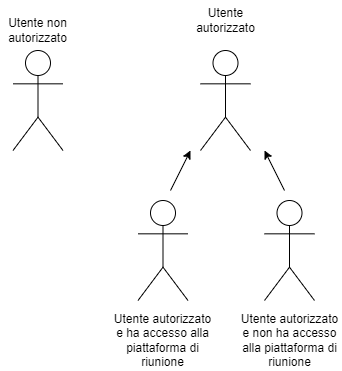
\includegraphics[scale=0.70]{images/Attori.png}
\end{center}
\newpage

\end{document}
